\chapter{Single User Interaktion}
\label{ch:Single_User_Interaktion}

\section{Realisierung}

\subsection{SteamVR-Plugin}
\label{ch:steamvr_plugin}

Für die Anbindung der VR-Brille und der beiden Controller wurde das Unity Plugin SteamVR verwendet (\cite{noauthor_steamvr_2019}). Das SteamVR Plugin beinhaltet verschiedene vorgefertigte Objekte, auch Prefabs genannt, welche dem Programmierer den Einstieg und die Arbeit mit Virtual Reality in Unity erleichtern. Eines dieser Prefabs namens \grqq Player\grqq{} ist dafür da, die VR-Brille mitsamt den beiden Controllern in Unity abzubilden, so dass diese ohne weiteres verwendet werden können. 
Das verwendete \grqq Player\grqq-Prefab beinhaltet die folgenden Punkte, um welche sich der Programmiere nicht mehr kümmern muss:

\begin{itemize} [itemsep=1pt,topsep=0pt]
	\item Regelt die Inputs der Controller und generiert daraus Events, auf welche der Programmierer sich abonnieren kann
	\item Handhabt die Kamera
	\item Zeichnet die Grenzen der virtuellen Umgebung, in welcher der Spieler sich sicher bewegen kann, ohne in der realen Welt in ein anderes Objekt zu laufen
\end{itemize}
 

\subsection{Highlight}
\label{ch:highlight_realisierung}
Dank der Beispiel Szene im SteamVR Asset, beschrieben im Kapitel \ref{ch:highlight}, war sehr schnell klar, wie das Highlight der Objekte im Asset selbst gemacht wird. Um die Silhouette des Objektes gelb umrahmen zu können, wird das Material aller MeshRenderer (in Unity zuständig für die visuelle Darstellung eines GameObjects) des Objektes ersetzt, mit einem Material, auf welchem sich ein spezifischer Shader befindet. Dieser Shader zeichnet nur die Aussenlinie des Meshes und macht alles innerhalb dieser Linie transparent. Um die originale Farbe des Objektes nicht zu verlieren, wird das Objekt erst kopiert und anschliessend das Material auf dem kopierten Objekt geändert. Die Kopie des Objektes muss erstellt werden, da das originale Material beibehalten werden soll. Würde das Material direkt auf dem Objekt angepasst, würde nur noch die gelbe Aussenlinie zu sehen sein. Diese Lösung ist sehr ineffizient und könnte besser gelöst werden. Mehr dazu im Kapitel \ref{ch:Ausblick}. \\

\noindent Das Highlight in der Single-User Applikation wurde genau wie im vorherigen Abschnitt beschrieben implementiert. An den beiden Controllern des Benutzers wurde jeweils ein Trigger hinzugefügt. Ein Trigger ist ein Collider, welcher aber keine Kollision verursacht sondern lediglich ein Event feuert, sobald er mit einem anderen Collider oder Trigger in Berührung kommt. \\
Dieses Event wird von der Applikation abgefangen und löst das Highlight des kollidierten Objektes aus. Dies ist in Abbildung \ref{fig:highlight_single_user_application} dargestellt.

\begin{figure}[h!]
	\centering
	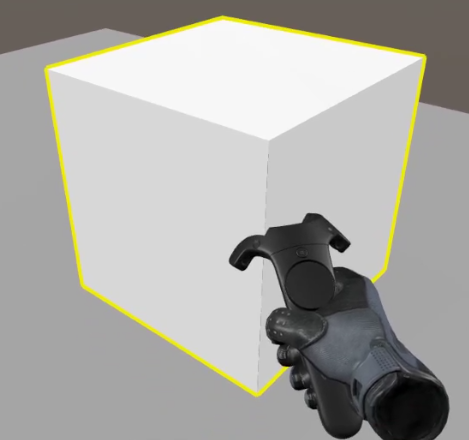
\includegraphics[keepaspectratio,width=0.4\linewidth]{img/Single_User_Highlight.PNG}
	\caption{Highlight in der Single User Applikation}
	\label{fig:highlight_single_user_application}
\end{figure}

\subsection{Snapping}
\label{ch:snapping}
Zwischen den Bauteilen, bei welchen das Snapping stattfinden soll, wurden Trigger angebracht, welche genau aufeinander passen (Abbildung \ref{fig:trigger_between_objects}). Sobald sich diese Trigger berühren wird ein Event ausgelöst, welches das Bauteil in der Hand des Benutzers als Silhouette am vorgesehenen Ort zeichnet (Abbildung \ref{fig:snapping}). \\
Dafür wird eine Kopie des Bauteils mitsamt dem Trigger erstellt, so positioniert, dass die beiden Trigger übereinstimmen und anschliessend das Material durch den Highlight-Shader ersetzt (beschrieben in Kapitel \ref{ch:highlight_realisierung}).

\begin{figure}[h!]
	\centering
	\begin{minipage}[b]{0.49\linewidth}
		\centering
		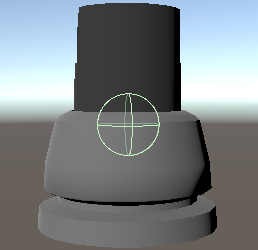
\includegraphics[keepaspectratio,width=0.9\linewidth]{img/Trigger_Between_Objects.PNG}
		\caption{Trigger zwischen Bauteilen}
		\label{fig:trigger_between_objects}
	\end{minipage}
	\hfill
	\begin{minipage}[b]{0.49\linewidth}
		\centering
		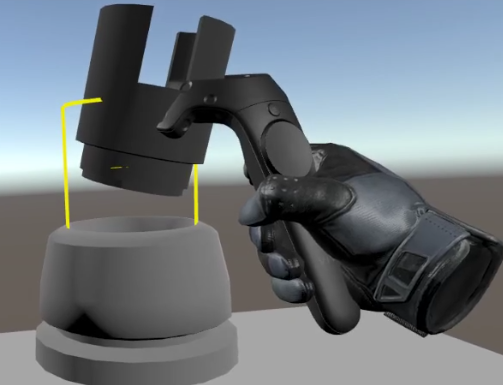
\includegraphics[keepaspectratio,width=0.9\linewidth]{img/Snapping.PNG}
		\caption{Highlight des Snappings}
		\label{fig:snapping}
	\end{minipage}
\end{figure}

\subsection{Kollision}
\label{ch:kollision_single_user}
Falls das Bauteil, wie in Kapitel \ref{ch:kollision} beschrieben, nur von der Hand losgelöst wird, kann es nicht ohne weiteres wieder an die Hand des Benutzers gemacht werden beim verlassen der Kollision. Auch andere Ansätze funktionierten nicht direkt so wie gedacht. \\

\noindent Um die Kollision der Bauteile so natürlich wie möglich zu machen, mussten den Bauteilen ein Rigidbody angehängt werden. Dieser ist für die Physik-Berechnungen zuständig und kann konstante Beschleunigungen oder eine konstante Geschwindigkeit auf das Bauteil geben. Sobald nun zwei Bauteile kollidieren, wird dem Rigidbody auf dem Bauteil, welches sich aktuell an der Hand des Benutzers befindet, mitgeteilt, dass es nicht mehr Kinematisch sein soll. Damit wird bewirkt, dass dieses Bauteil sich mithilfe der Physik bewegen kann (Die Gravitation ist deaktiviert). Da das Bauteil so aber langsam in eine Richtung gleiten würde, muss ihm eine konstante Geschwindigkeit zum Controller hin gegeben werden. Die Geschwindigkeit errechnet sich durch die Distanz des Bauteils zum Controller des Benutzers. Diese Distanz ist ein dreidimensionaler Vektor, welcher in eine bestimmte Richtung zeigt. Das heisst, dass der Vektor grösser wird umso grösser die Distanz zwischen dem Bauteil und dem Controller wird. Sobald das Bauteil mit keinem anderen Bauteil mehr kollidiert, wird der Rigidbody wieder Kinematisch und die Geschwindigkeit auf null gesetzt. Dieses Verhalten ist in Abbildung \ref{fig:collision} dargestellt.

\begin{figure}[h!]
	\centering
	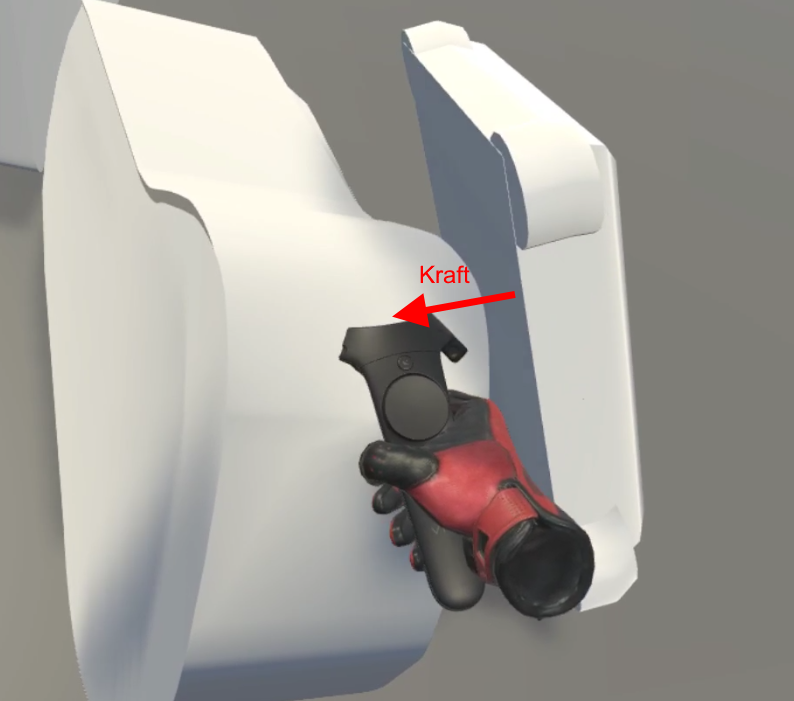
\includegraphics[keepaspectratio,width=0.4\linewidth]{img/Kollision.PNG}
	\caption{Kollision zwischen zwei Objekten und der konstanten Kraft}
	\label{fig:collision}
\end{figure}

\subsection{Baugruppen}
\label{ch:baugruppen}
Während der Arbeit wurde bemerkt, dass es sehr umständlich sein kann, mehrere Bauteile miteinander zu transportieren. Alle Bauteile mussten an einem Ort auseinandergenommen werden nur um diese an einem anderen Ort wieder zusammenzubauen. Um dies zu erleichtern wurde jedem Bauteil eine Liste von Kindern angehängt, welche besagt, welche Bauteile mit dem aktuellen Bauteil mitbewegt werden sollen. Dies resultiert darin, dass es bei jeder Maschine ein Bauteil gibt, an welchem alle anderen Bauteile direkt oder indirekt über andere Bauteile befestigt sind.

Um dem Benutzer mitteilen zu können, in welcher Situation er welche Bauteile zusammen bewegen kann, wurde das Highlight, beschrieben in Kapitel \ref{ch:highlight_realisierung}, wie folgt angepasst. Für jedes Kind des Bauteils wurde überprüft, ob es zum aktuellen Zeitpunkt verbunden ist und falls dies der Fall ist, wird auch von diesem Bauteil eine Kopie erstellt und der Shader für das Highlight hinzugefügt. Somit werden alle Bauteile, welche miteinander bewegt werden können, wie in Abbildung \ref{fig:highlight_baugruppe} ersichtlich, mit einem Highlight versehen.

\begin{figure}[h!]
	\centering
	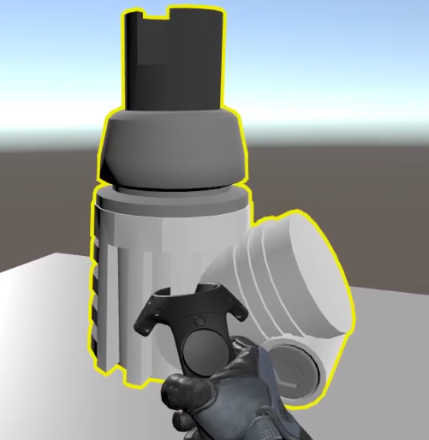
\includegraphics[keepaspectratio,width=0.37\linewidth]{img/Baugruppe_Highlight.PNG}
	\caption{Highlight einer Baugruppe}
	\label{fig:highlight_baugruppe}
\end{figure}

\subsection{Feedback beim Zusammenbau / Manipulation der Objekte}
\label{ch:feedback_zusammenbau_manipulation}

Da drei verschiedene Varianten, beschrieben in Kapitel \ref{ch:feedback_zusammenbau_konzepte}, implementiert wurden, wurde für jede Variante ein eigener Prototyp mit einer eigenen Maschine erstellt. \\

\noindent Die Variante, bei welcher dem Benutzer ein visuelles Feedback gegeben wird, wurde wie folgt implementiert. Bei einer Kollision zwischen zwei Bauteilen, wird das Bauteil in der Hand des Benutzers, wie in Abbildung \ref{fig:kollision_variante_1} zu sehen, rot eingefärbt. Sobald die Kollision endet, wird die Farbe des Bauteils wiederhergestellt.

\begin{figure}[h!]
	\centering
	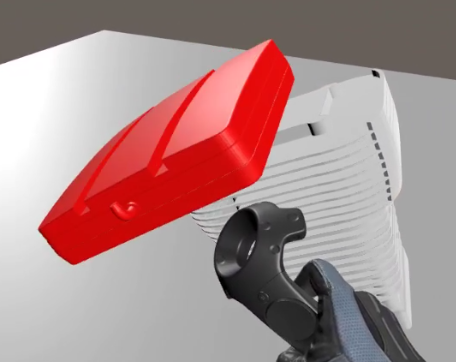
\includegraphics[keepaspectratio,width=0.37\linewidth]{img/Kollision_Variante1.PNG}
	\caption{Visuelles Feedback bei einer Kollision}
	\label{fig:kollision_variante_1}
\end{figure}

Für die Umsetzung der zweiten Variante, bei welcher die Freiheitsgrade des Benutzers eingeschränkt werden, wurde die Ausrichtung des Triggers verwendet, welcher für das Snapping gebraucht wird. Sobald sich das Bauteil im Bereich des automatischen Snappings befindet, wird das Bauteil in der Hand des Benutzers anhand des Triggers ausgerichtet. Zur gleichen Zeit wird zwischen den beiden Bauteilen ein Joint platziert. Ein Joint ist eine Verbindung zwischen zwei Bauteilen und hat je nach Art des Joints unterschiedliche Eigenschaften. Im Falle dieser Applikation wird ein Joint verwendet, bei welchem zwei Achsen sowie die Rotation in allen Achsen fixiert werden. Somit lässt sich das Bauteil, wie in Abbildung \ref{fig:einschraenkung_freiheitsgrade} zu sehen, nur noch auf einer Achse bewegen.

\begin{figure}[h!]
	\centering
	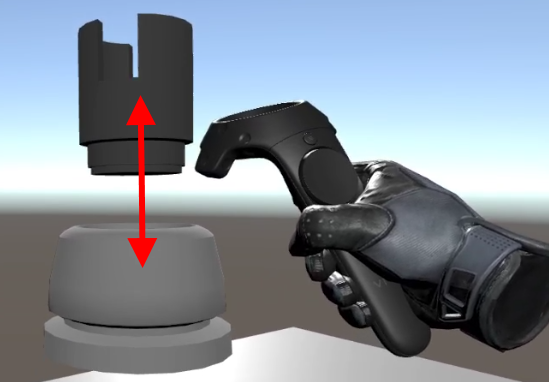
\includegraphics[keepaspectratio,width=0.4\linewidth]{img/Einschraenkung_Freiheitsgrade.PNG}
	\caption{Einzige bewegbare Achse durch die Einschränkung der Freiheitsgrade}
	\label{fig:einschraenkung_freiheitsgrade}
\end{figure}

Die dritte Variante, mit dem Vibrations Feedback, konnte mithilfe des SteamVR Assets implementiert werden. Um auf die Vibration des Controllers zugreifen zu können, muss lediglich bekannt sein, auf welchem Controller die Vibration ausgeführt werden soll. Die Übergabeparameter der Funktion des SteamVR Assets erlauben dann die Vibration wie folgt anzupassen:

\begin{itemize} [itemsep=1pt,topsep=0pt]
	\item Startzeit der Vibration in Sekunden ab dem aktuellen Zeitpunkt
	\item Dauer der Vibration
	\item Frequenz der Vibration in Hertz
	\item Stärke der Vibration
\end{itemize}

\pagebreak
\section{Evaluation}
Nach Abschluss der Realisierungsphase des Single-User Prototypen wurde eine Nutzerevaluation durchgeführt um den Prototypen zu evaluieren und um entscheiden zu können, welcher der drei beschrieben Varianten in Kapitel \ref{ch:feedback_zusammenbau_manipulation} sich für diese Applikation am besten eignet. 


\subsection{Aufgabenstellung}
Während der Nutzerstudie mussten die Teilnehmer zwei Aufgaben erledigen. Bei beiden Aufgaben wurden ihnen drei Maschinen gezeigt, mit jeweils einer anderen Art des Feedbacks beim Zusammenbau / Manipulation der Objekte.
\begin{enumerate}
	\item In der ersten Aufgabe ging es darum, eine Maschine zusammenzubauen, welche sich in einer explosionsartigen Darstellung vor dem Nutzer befand. 
	
	\begin{figure}[h!]
		\centering
		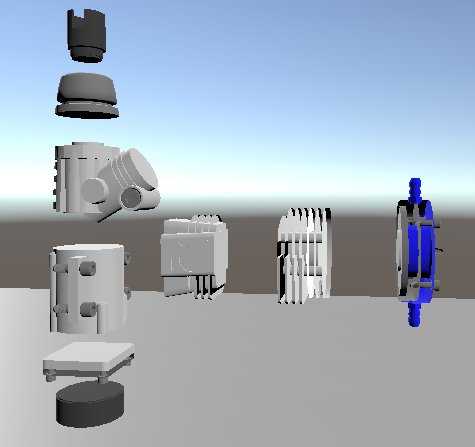
\includegraphics[keepaspectratio,width=0.35\linewidth]{img/Evaluation_Task1.PNG}
		\caption{Erste Aufgabe der ersten Nutzerevaluation}
		\label{fig:evaluation1_task1}
	\end{figure}
	
	\item Die zweite Aufgabe bestand darin, ein rot eingefärbtes Bauteil aus der Maschine auszubauen, dieses in einen gelben Bereich zu halten, um es automatisch reparieren zu lassen, und anschliessend dieses nun grün gefärbte Bauteil wieder in der Maschine einzubauen.
	
	\begin{figure}[h!]
		\centering
		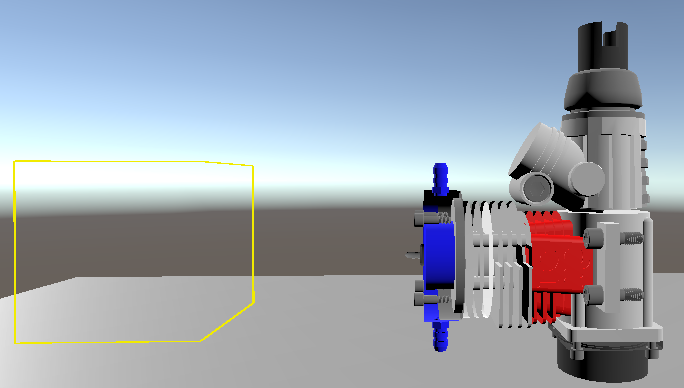
\includegraphics[keepaspectratio,width=0.45\linewidth]{img/Evaluation_Task2.PNG}
		\caption{Zweite Aufgabe der ersten Nutzerevaluation}
		\label{fig:evaluation1_task2}
	\end{figure}
	
\end{enumerate}

\pagebreak
\subsection{Resultat}
Insgesamt haben sechs Teilnehmer an der Nutzerevaluation teilgenommen. Alle Teilnehmer hatten bereits Erfahrungen mit Virtual Reality. \\

\noindent Den Teilnehmern wurden nach dem Abschluss der Aufgaben die folgenden fünf Fragen gestellt:

\begin{enumerate} [itemsep=2pt]
	\item Frage: Wie empfanden Sie die Steuerung mit dem Kontroller? \\
	Auswertung: Die Teilnehmer fanden die Steuerung mit dem Controller sehr angenehm und intuitiv. Nur eine Person bemängelte, dass die verwendeten Buttons beschriftet hätten sein müssen um die Interaktion noch klarer zu machen.
	
	\item Frage: Wie verständlich ist die Manipulation der Objekte? \\
	Auswertung: \grqq Man wusste immer mit welchem Objekt man interagiert\grqq{}, meinte einer der Testpersonen. Dies fasst ziemlich gut die allgemeine Rückmeldung zur Manipulation der Objekte zusammen.
	
	\item Frage: Was hat Ihnen an der Applikation besonders gefallen? \\
	Auswertung: Das Highlight sowie das Snapping hat sehr vielen Teilnehmern besonders gefallen. Zwei Teilnehmer haben geschrieben, dass ihnen das einfach gehaltene Interface sowie die einfache Handhabung der Applikation gut gefallen hat.
	
	\item Frage: Wie natürlich empfanden Sie die Interaktion mit den Objekten? \\
	Auswertung: Die Teilnehmer fanden die Interaktion mit den Objekten sehr natürlich. Dank den Features wie das Snapping, die Baugruppen und das Highlight fiel es den Teilnehmern sehr leicht mit den Objekten zu interagieren und dementsprechend wirkte die Interaktion natürlicher.
	
	\item Frage: Welche Variante der Rückmeldung einer nicht erlaubten Bewegung hat Ihnen am besten gefallen und wieso? \\
	Auswertung: Fünf von den sechs Teilnehmern fanden die Variante mit dem Vibrations-Feedback am besten geeignet für diese Applikation. Es sei die natürlichste Variante und der Benutzer bemerke eine unerlaubte Bewegung auch dann, falls er das Bauteil gerade nicht im Blickfeld hat. \\
	Die Variante mit dem Einfärben der Bauteile passe nicht. Möglicherweise wurde die Farbe falsch gewählt und deswegen erscheine es unnatürlich, meinten zwei Teilnehmer. \\
	Die dritte Variante, bei welcher die Freiheitsgrade eingeschränkt wurden, könnten sich zwei Teilnehmer bei gewissen Teilen der Applikation vorstellen. \grqq Beim Anbringen einer Schraube könnte ich mir diese Variante mit den Freiheitsgraden vorstellen\grqq{}, meinte einer dieser beiden Teilnehmern. Der andere schrieb, dass er sich eine Kombination der beiden Varianten vorstellen könnte: \grqq Kombination von Variante 1 und 2 würde gut passen. Weiter weg zum fahren, sobald nah genug dann Snapping und je nachdem Vibration.\grqq{}
\end{enumerate}

\pagebreak
\subsection{Schlussfolgerung}
\label{ch:schlussfolgerung_t1}
Die Teilnehmer der Nutzerevaluation waren sehr zufrieden mit dem Single-User Prototyp. Bemängelt wurde einzig die Implementation der Variante, bei welcher die Freiheitsgrade der Benutzer eingeschränkt wird. Diese Variante hatte öfters Probleme, da sich die Objekte anders verhalten hatten als sie sollten oder diese gar in der Szene umhergesprungen sind. Dementsprechend ist die Bewertung dieser Variante insgesamt schlechter ausgefallen. Bei der Variante, bei welcher die Bauteile eingefärbt werden wurde vermutlich die Farbe falsch gewählt. Das rot symbolisierte eher, dass etwas falsche gemacht wurde, anstatt der Kollision mit anderen Bauteilen. Mit einer anderen Farbwahl, oder einer transparenteren Farbe, hätte die Nutzerevaluation eventuell anders ausfallen können. \\

\noindent Die meisten Teilnehmer fanden die Vibrations-Feedback Variante am besten geeignet für diese Applikation. Dementsprechend wird diese Variante für den zweiten Prototypen verwendet. Falls es die Zeit zulässt, könnte sich überlegt werden, gewisse Bauteile, wie zum Beispiel Schrauben, mit der Kombination von Vibration und Einschränkung der Freiheitsgrade zu implementieren.

\section{Systemarchitektur}
\label{ch:systemarchitektur_single_user}
\begin{figure}[h!]
	\centering
	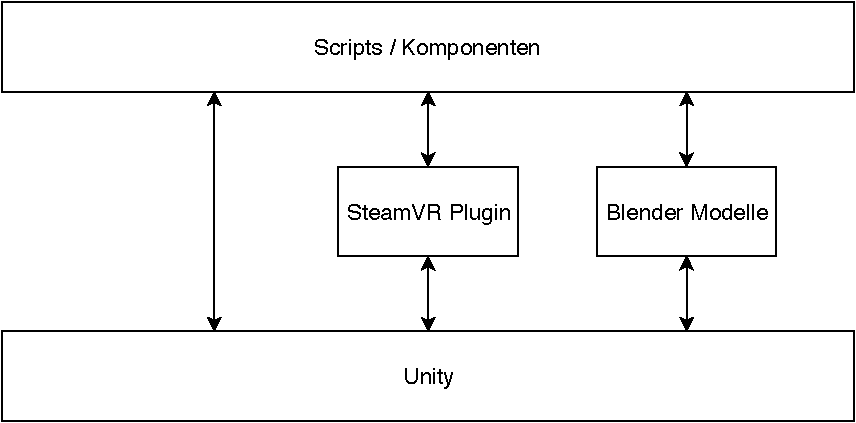
\includegraphics[keepaspectratio,width=0.65\linewidth]{img/ArchitekturT1.pdf}
	\caption{Systemarchitektur des Single-User Prototypen}
	\label{fig:systemarchitektur_single_user}
\end{figure}

Die Systemarchitektur des Single-User Prototypen ist in Abbildung \ref{fig:systemarchitektur_single_user} dargestellt. Als Basis dient die Game-Engine Unity und alle zur Verfügung gestellten Features. Das für die Virtual Reality Anbindung verwendete SteamVR Plugin kommuniziert mit Unity und stellt eine Schnittstelle für eigene Skripte dar. Die 3D Modelle werden von Unity importiert und in ein nutzbares Format innerhalb von Unity konvertiert. \\
Die erstellten Skripte und verwendeten Komponenten, beschrieben in Kapitel \ref{ch:klassendiagram_single_user}, befinden sich auf den konvertieren 3D Modellen oder verwendeten SteamVR Komponenten. Die Skripte verwenden Funktionen des SteamVR-Plugins und von Unity selbst.


\section{Klassendiagramm}
\label{ch:klassendiagram_single_user}

\begin{figure}[h!]
	\centering
	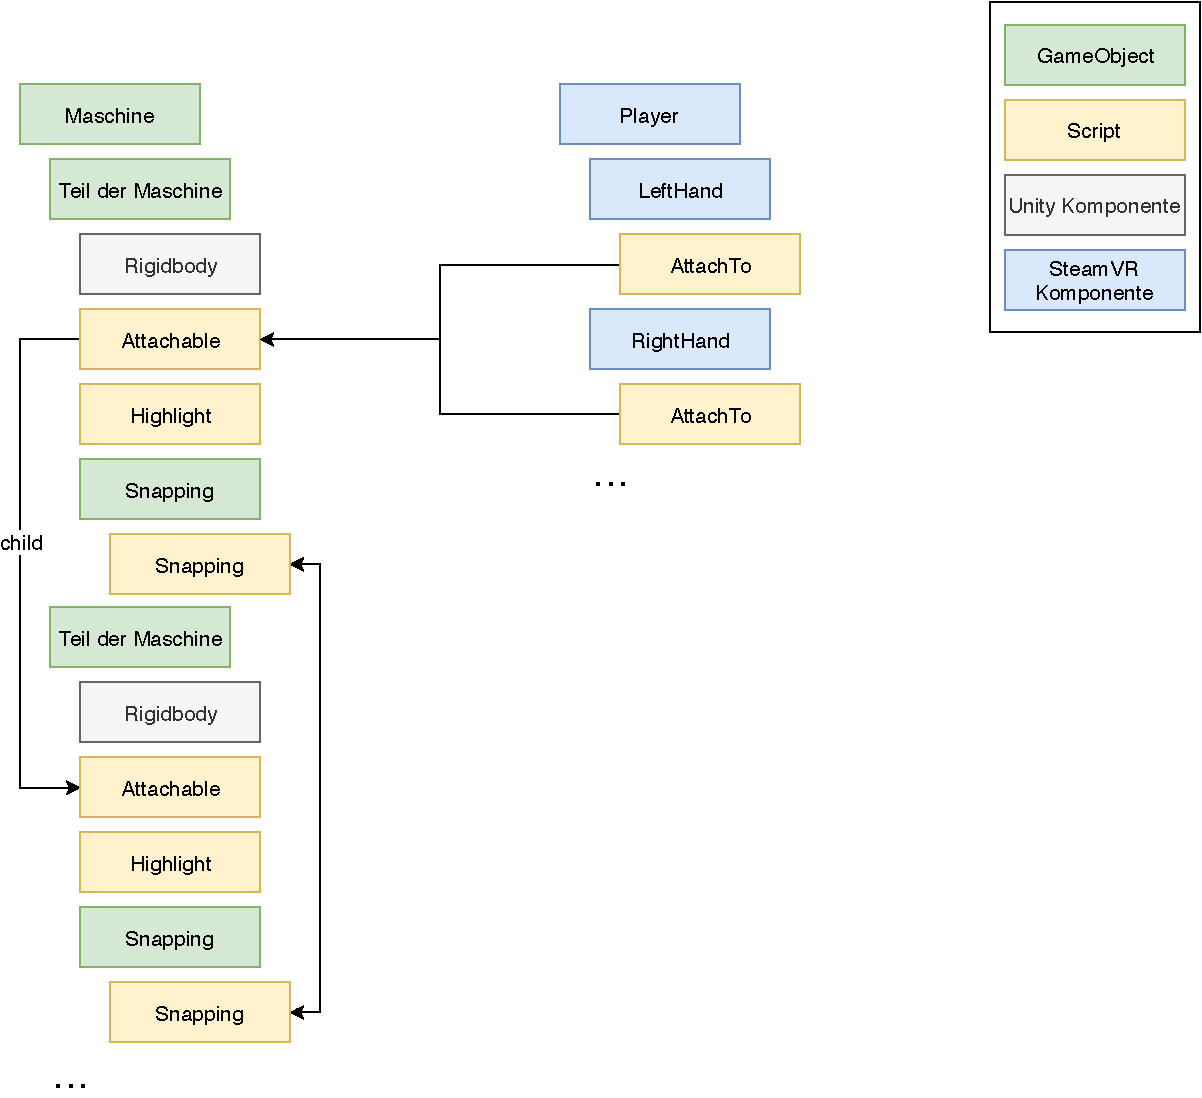
\includegraphics[keepaspectratio,width=0.75\linewidth]{img/Klassendiagramm_T1.pdf}
	\caption{Klassendiagramm des Single-User Prototypen}
	\label{fig:klassendiagramm_single_user}
\end{figure}

Der \grqq Player\grqq{} ist ein Prefab, welches vom SteamVR-Plugin zur Verfügung gestellt wird, beschrieben in Kapitel \ref{ch:steamvr_plugin}. An diesem Prefab wurde lediglich der linken und rechten Hand ein Skript \grqq AttachTo\grqq{} hinzugefügt. Dieses Skript fängt die Inputs des Benutzers ab und teilt beim Greifen eines Objektes dem \grqq Attachable\grqq{} Skript mit, dass es nun gegriffen wurde. \\

\noindent Die Maschine wurde in verschieden Teile unterteilt, jeder Teil der Maschine kann bewegt und auseinandergenommen werden. Die Funktionalität der Skripts wurde in folgenden Kapiteln beschrieben:

\begin{itemize} [itemsep=1pt,topsep=0pt]	
	\item Highlight: Zuständig für das Highlight der Bauteile, falls sich eine Hand des Benutzers in einem Bauteil befindet sowie das Highlight des Snappings. Beides ist beschrieben im Kapitel \ref{ch:highlight_realisierung}.
	
	\item Snapping: Zuständig für das Snapping der Bauteile, beschrieben in Kapitel \ref{ch:snapping}.
	
	\item Attachable: Zuständig für das Kollidieren der Bauteile, beschrieben in Kapitel \ref{ch:kollision_single_user}, für die Baugruppen, beschrieben in Kapitel \ref{ch:baugruppen} und das Feedback beim Zusammenbau, beschrieben in Kapitel \ref{ch:feedback_zusammenbau_manipulation}.
\end{itemize}